\documentclass{article}

\usepackage{graphicx}

\title{MSPMeter: Software Architecture}
\author{Joris Gillis}

\begin{document}

\maketitle


\section{Introduction}

This document describes the overall software architecture of MSPMeter. The software is modeled as a collection of cells. There is a cell for each element of the input, i.e., a cell for the input files, a cell for the sample size, a cell for each version of MSP (weighted vs unweighted and entropy versus frequency, cumulative, etc). Basically, there is a cell for each element of the graphical user interface (GUI). The second type of cells are the ``internal cells''. These cells contain intermediate values, for example, the data with lemma equivalences applied. Last but not least, there are output cells linked to the output widgets of the GUI. 

Cells on their own are only useful for storing information. The computation arises if cells are connected in a network. The connections between cells are asymmetric (or directed), i.e., if cell A is connected to cell B, a change in cell A is reported to cell B, but a change in cell B is not reported to cell A. Cell B can distinguish signals from different cells, and has ``handlers'' for each signal. For example, if cells A and B are connected to cell C, a change in cell A can trigger a different mutation of the information stored in cell C then a change in cell B. 


\section{Data Cube}

The data on which MSPMeter works is represented by a three-dimensional cube, called \emph{data cube}.  The first dimension of the cube is the ``age'', as defined by the user by inputting files. We will call this the \emph{span-dimension}, as it is defined by the spans. The second dimension consists of all the lemmas in all files. The third dimension is made up of categories. If there are no categories defined in the data, a default category is introduced, i.e.\ the data cube becomes a data plane. 

The \texttt{DataCube} class is essential in the design of MSPMeter. It contains the data and the functions to manipulate the data (e.g.\ sampling, calculating properties of the data necessary to compute the MSP, etc).


\section{The Grid}

In this section we give a listing of all cells present in the grid of MSPMeter. An overview of the cells and their connection is shown in Figure~\ref{fig:cells}. The square boxes denote information in the grid from the GUI. Round nodes represent internal data, not visible to the user. The rhombus-shaped nodes in the graph are  output widgets in the GUI, i.e.\ they represent information/data to the user. 

Notice that some connections (i.e.\ arrows) are colored red. This are ``hot flows", implying that if a cell changes, it changes is reported automatically to all dependent cells. Almost all input-cells are hot flowing, up to the results cell. Because the actual MSP calculation is fairly computationally heavy, it is postponed until the Results pane is reached, or the user instructs the program to compute. Therefore, we call the black connections ``cold flowing''. They only flow when demanded. Another way of looking at hot and cold flowing is in terms of ``eager'' and ``lazy'' connections.

\begin{figure}[t]
	\begin{center}
	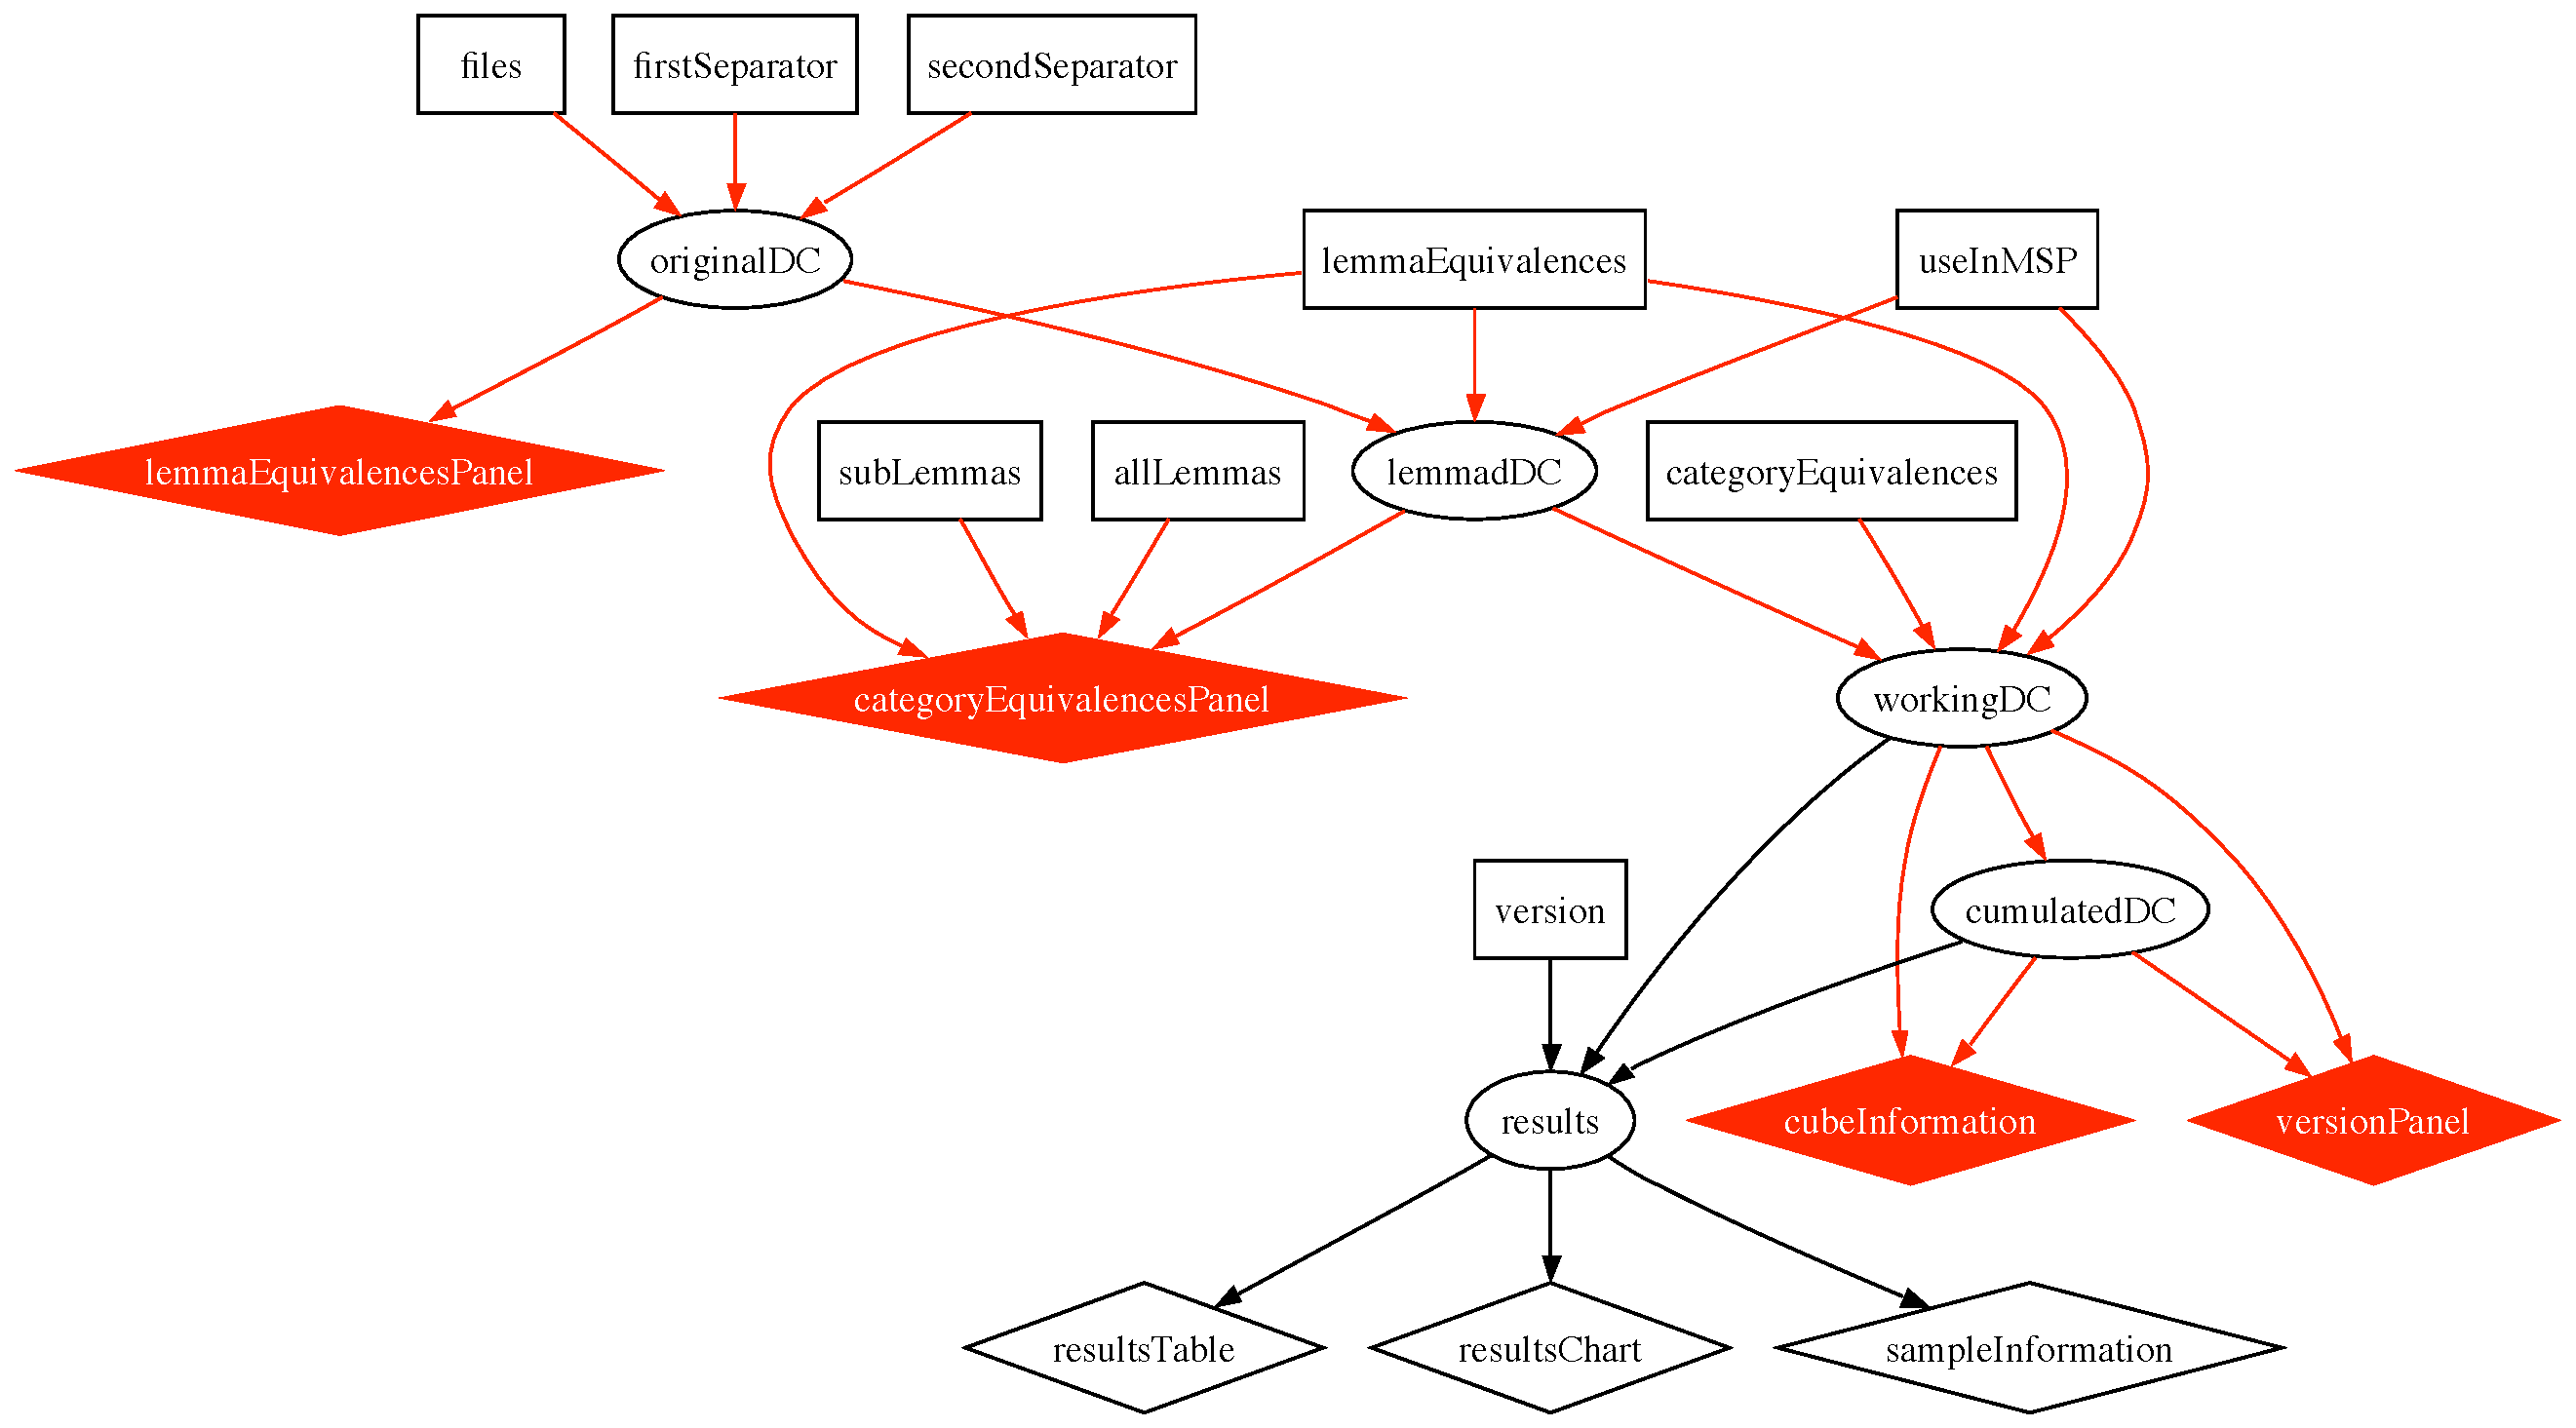
\includegraphics[scale=0.3]{dataflow}
	\caption{An overview of the cells and connections between the cells of MSPMeter.  \label{fig:cells}}
	\end{center}
\end{figure}


An overview of all cells:
\begin{description}
\item[\texttt{files}] Contains an ordered list of spans. A \emph{span} is a set of files, together making up a logic unit the development of a child. For example, the speech of a child is recorded several times each month. All sessions recorded in one month are then bundled in a single span. 

\item[\texttt{firstSeparator}] Equals the value entered in the ``Token indicating lemma:''-field in the GUI. The characters entered in this field indicate the start of a lemma.

\item[\texttt{secondSeparator}] Equals the value entered in the ``Token between lemma and category:''-field in the GUI. The characters entered in this field indicate the separation between lemma and category. 

\item[\texttt{originalDC}] Is the data cube constructed by taking the files from the \texttt{files} cell and the characters from the \texttt{firstSeparator} and \texttt{secondSeparator}. In other words, this data cube contains the unprocessed data.

\item[\texttt{lemmaEquivalencesPanel}] Uses the \texttt{originalDC} to generate a default set of lemma equivalences (namely every lemma has its own equivalence class). 

\item[\texttt{lemmaEquivalences}] The result of the lemma equivalences panel: a set of lemma equivalences. 

\item[\texttt{useInMSP}] Corresponds to the ``Use in MSP''-checkbox in the GUI. If the cell's value is True, the lemma equivalences are used during the computation of MSP. Otherwise, the lemma equivalences are ignored (not sure why I did this).

\item[\texttt{lemmadDC}] The original data cube with lemma equivalences applied. If no lemma equivalences are applied, this equals the value of \texttt{originalDC}.

\item[\texttt{allLemmas}] Contains the set of all lemmas present in the original DC. It receives it information from the \texttt{lemmaEquivalencesPanel}. 

\item[\texttt{subLemmas}] Contains for each lemma the sublemmas. It receives it information from the \texttt{lemmaEquivalencesPanel}.

\item[\texttt{categoryEquivalencesPanel}] The panel in which the category equivalences are loaded and edited. 

\item[\texttt{categoryEquivalences}] Contains the category equivalence classes. 

\item[\texttt{workingDC}] Contains the data cube on which MSPMeter will work. Depending on the availability of lemma and category equivalences this data cube equals either the original data cube, the lemma'd data cube (if only lemma equivalences are specified) or the lemma'd data cube with category equivalences applied (if category equivalences, and possibly lemma equivalences, have been set).

\item[\texttt{cumulatedDC}] Contains the data cube in which cumulation has been applied across the span-dimension. 

\item[\texttt{cubeInformation}] This panel contains all kinds of information about the working data cube and the cumulated data cube: like the total number of lemmas, the sizes of the spans, etc, both for the working and cumulated data.

\item[\texttt{versionPanel}] In this panel the user specifies the sampling strategy and which version of MSP is calculated. Therefore, we need information about the number of lemmas in the spans, both in the working and cumulated data cube.

\item[\texttt{version}] Contains the parameters for the calculating of the MSP. 

\item[\texttt{results}] Contains the MSP values and the standard deviations. 

\item[\texttt{resultsTable}] The table displaying the MSP values and the standard deviations.

\item[\texttt{resultChart}] The chart displaying the MSP values and the standard deviations.

\item[\texttt{sampleInformation}] Displays the MSP value for each sample of each span.
\end{description}



\section{Sampling}



\end{document}
